\chapter{Quantum technology}
\label{ch:quantum}

With the word \textbf{quantum} mechanics, we refer to an \textbf{area
of physics} where classical deterministic rules do not hold any more
(Schrödinger, Dirac, Heisenberg, \dots).

One of the fundamental principles in quantum mechanics is the
\textbf{Uncertainty Principle}, also known as Heisenberg's
Indeterminacy Principle. This principle limit the precision with which
certain pairs of physical properties, such as position and momentum,
can be measured simultaneously. The more precisely one property is
determined, the less precisely the other can be known. For example,
one can measure the position of a particle with high accuracy, but the
momentum and the direction of the particle will be uncertain.

Another key concept is \textbf{Quantum Superposition}, which refers to
the ability of a quantum system to exist in multiple states
simultaneously, since we are unable to measure with infinite precision
some properties. This superposition remains until a measurement is
performed, at which point the system collapses into a single state.
This idea is famously illustrated in the thought experiment involving
Schrödinger's cat, which is simultaneously alive and dead until
observed.

An experimental demonstration of quantum mechanics is seen in
\textbf{Young's Double-Slit Experiment}. In this setup, a beam of
light is directed at a barrier with two vertical slits. When the
photons are not measured, they exhibit an interference pattern on a
screen, demonstrating wave-like behavior and moving in
all possible directions with different probabilities. However, if individual
photons are measured as they pass through the slits, the interference
pattern disappears, and the photons behave like particles,
highlighting the principle of wave-particle duality in quantum
mechanics.

\section{Probabilistic interpretation of QM}

In quantum mechanics, particles are described by a \textbf{wave
function}, denoted as \(\Psi(x,t)\), where \(x\) represents the
position and \(t\) represents time. Unlike classical physics, which
defines the exact position and velocity of a particle, quantum
mechanics introduces a probabilistic framework.

The wave function \(\Psi(x,t)\) provides information about the
probability of observing a particle at a specific position \(x\) at a
given time \(t\). However, the wave function itself is not directly
observable. 

Ad you could have noticed, this behaviour of the particles is quite
different from traditional physics, which relies on determinisctic
behaviours.


\section{Quantum Entanglement}

\begin{boxH}
\textbf{Quantum entanglement} occurs when a group of particles (at
least two) is in a quantum state such that the state of each particle
cannot be described independently of the states of the others.
\end{boxH}
A state could persist then even if the particles are separated and are
moving in opposite directions. The entire system could be described as
a single, \textbf{global quantum state} that persists even when the
particles are separated by large distances.

Let's now make an example, think about two particles, \(A\) and \(B\),
that are entangled in such a way that their total spin is zero. If
particle \(A\) is measured and found to have a \textbf{clockwise
spin}, then particle \(B\), when measured, will be found to have a
\textbf{counterclockwise spin}. This correlation persists even if the
two particles are separated by vast distances, a phenomenon that seems
to suggest that information is transmitted faster than the speed of
light.

However, this phenomenon does not violate the principles of
relativity. The reason is that, while the measurement of \(A\)
determines the state of \(B\), it is not possible to use this effect
to transmit information. The spin of \(A\) cannot be controlled or
predetermined, meaning no usable signal can be sent via entanglement.
This subtle distinction ensures that entanglement remains consistent
with the fundamental limits of information transfer imposed by the
speed of light.

\subsection{The No-Cloning Theorem}

The \textbf{no-cloning theorem} is a fundamental principle in quantum
mechanics stating this: 
\begin{boxH}
  it is \textbf{impossible to create an independent and identical copy
  of an arbitrary unknown quantum state}.
\end{boxH}
This theorem has profound implications for quantum information theory
and quantum cryptography, as it guarantees the security of quantum
communication protocols.

It is important to emphasize the role of \textbf{independence} in this
context. While entanglement allows for correlations between particles,
it does not enable the independent duplication of a quantum state. The
inability to clone quantum states arises from the linearity of quantum
mechanics and the fact that measurement collapses a quantum state,
making it impossible to perfectly reproduce its original form. This
principle underpins the security of quantum key distribution (QKD)
systems, such as those based on the BB84 protocol.

\section{Quantum Computing}

Is it different from classical computing?  The short answer is yes. 
Quantum computing introduces a fundamentally different approach to
computation compared to classical computing. While classical computers
rely on binary bits (0 or 1) to process information, quantum computers
use \textbf{qubits} that leverage unique quantum properties to achieve
greater computational power. The key differences are explained through
the following concepts:

\paragraph{Quantum Superposition}  
Unlike classical bits, qubits can exist in a \textbf{superposition} of
0 and 1 simultaneously. This allows a quantum computer to explore
multiple states at once, effectively processing many possible outcomes
in parallel. This parallelism provides quantum computers with a
significant speed advantage for certain types of problems.

\paragraph{Quantum Entanglement}  
Quantum entanglement allows qubits to be \textbf{correlated} with each
other, even when they are physically separated. This enables
coordinated processing and allows the system to perform more complex
calculations efficiently. Entanglement is a crucial feature that
enables the development of quantum algorithms like Grover's search
algorithm and Shor's factoring algorithm.

\paragraph{Quantum Interference}  
Quantum computers exploit \textbf{constructive and destructive
interference} to enhance the probabilities of correct answers while
cancelling out incorrect ones. By carefully designing quantum
algorithms, the probabilities of "correct paths" are amplified,
allowing the quantum computer to find the right solution more
efficiently than classical methods.

These features collectively enable quantum computers to solve certain
classes of problems exponentially faster than classical computers,
such as factoring large numbers, optimizing complex systems, and
searching unstructured databases.

On the other hand, QC are not a general-purpose technology. They only
works on specific classes of problems, where the quantum effects can
be exploited (e.g. superposition). 

Currently, one of the most successful applications of quantum
computing is in \textbf{optimization problems}. In this domain,
\textbf{Quantum Annealing (QA)} has proven effective. Quantum
annealers, like those produced by \textbf{D-Wave Systems}, are
special-purpose quantum devices. They employ \textbf{adiabatic quantum
computation} and are based on superconducting technology to solve
large-scale optimization problems. Unlike general quantum computers,
quantum annealers are tailored to address specific optimization tasks.

Quantum computing faces significant challenges related to
manufacturing and operational constraints. For instance, the
\textbf{D-Wave 2X} quantum annealer, released in 2015, was equipped
with \textbf{1152 qubits}. However, due to \textbf{manufacturing
variability}, not all qubits are functional, and the exact number of
usable qubits varies across individual processors. This variability
highlights the complexity of producing reliable and consistent quantum
processors. The use of superconducting technology also introduces
environmental constraints, such as the need for ultra-low temperatures
for stable operation.

\section{The quantum problem for cryptography}
The main problem is that the current cryptographic algorithms have an
expiration data. Think for example about the DES algorithm, which was
once considered state of the art, but now is considered insecure.

Currently, the Global Risk Institute estimated that in 15-30 years, a
sufficiently powerful QC will be built, able to decrypt ANY encrypted
data on the Internet today. This is a huge deal for the future, but
it's also a problem nowadays, because attackers are harvesting data
today to decrypt it in the future. This approach assumes that the data
still holds some value in the future, which is not true for most data,
but if you think about state secrets, you can see that they a much
longer expiration date. 

This is something that is happening nowadays, as states are collecting
data in large data centers, and they are storing it for future use.
Wikileaks disclosed that there is a global network named X-Keyscore,
in which there are servers installed in about 150 sites for a total of
over 700 servers that are continuously copying all the internet data.

\subsection{Security of current cryptography}
The security of modern cryptography is founded on a combination of
\textbf{mathematically hard problems}, which are non polinomial, and
the \textbf{impracticality of exhaustive search}. These principles
underpin the two main types of cryptographic methods: asymmetric
cryptography and symmetric cryptography.

\paragraph{Mathematically Hard Problems}  
Asymmetric cryptographic systems, such as those used in
\textbf{digital signatures} and \textbf{key exchange protocols}, rely
on computational problems that are considered \textbf{NP-hard}. The
most common of these problems are:  
\begin{itemize}
  \item \textbf{Discrete Logarithm Problem}: Used in cryptographic
    schemes involving \textbf{integers} or \textbf{elliptic curves}
    (e.g., ECDSA, ECDH). Solving the discrete logarithm problem
    efficiently is considered infeasible with current classical
    computational methods.  
  \item \textbf{Integer Factorization Problem}: The basis of
    \textbf{RSA cryptography}, where the security of the system
    depends on the difficulty of factoring large composite numbers
    into their prime factors.  
\end{itemize}

Symmetric cryptographic systems, such as those used for
\textbf{encryption} (e.g., AES) and \textbf{hashing} (e.g., SHA-256),
derive their security from the sheer size of the \textbf{key space}.
Unlike asymmetric systems, these methods rely on the infeasibility of
performing an exhaustive search over all possible key combinations
within a reasonable timeframe. For instance, a 128-bit key has
$2^{128}$ possible combinations, making brute-force attacks
computationally infeasible.  

By leveraging these two core principles — reliance on NP-hard problems
and the infeasibility of exhaustive search — modern cryptographic
systems maintain a high level of security against classical
computational attacks.

\subsubsection{DH, RSA, and Quantum Computing}

\paragraph{Diffie-Hellman (DH)}  
The security of the \textbf{Diffie-Hellman (DH) key exchange} is
rooted in the computational complexity of the \textbf{Discrete
Logarithm Problem}. Given an equation of the form  
\[
A = g^x \mod p
\]  
where \(g\) is the generator, \(p\) is a large prime, and \(A\) is a
known value, the challenge is to find \(x\). This requires solving  
\[
x = \log_g A \mod p
\]  
which is computationally hard. The simplest attack is to try all
possible values of \(x\), which takes time linear in \(p\). Since
\(p\) is often a large prime (e.g., 2048 bits), this time complexity
is exponential in the bit-length of \(p\).  

\paragraph{Efficient Algorithms for Discrete Logarithm}  
While a brute-force search for \(x\) is infeasible, more advanced
algorithms exist that reduce the computational complexity, although
they still remain non-polynomial. These include:  
\begin{itemize}
    \item \textbf{Pohlig-Hellman Algorithm}: Breaks the problem into
      smaller sub-problems using the factorization of \(p-1\).  
    \item \textbf{Number Field Sieve (NFS)}: One of the most efficient
      known methods for solving discrete logarithms in large finite
      fields.  
\end{itemize}

\paragraph{RSA and Factorization}  
The security of \textbf{RSA} encryption and signatures relies on the
difficulty of \textbf{integer factorization}. Similar to the discrete
logarithm, factorization is computationally infeasible for large
integers composed of two large prime factors. The link between DH and
RSA is that the mathematical techniques used to solve the discrete
logarithm can often be adapted for integer factorization, and vice
versa. However, there are also specialized factorization algorithms,
such as:  
\begin{itemize}
    \item \textbf{Elliptic Curve Method (ECM)}: Useful for factoring
      large numbers with small prime factors.  
    \item \textbf{General Number Field Sieve (GNFS)}: The most
      effective classical algorithm for factoring large integers.  
\end{itemize}

\section{Shor's algorithm}
\textbf{Shor's algorithm}, developed by Peter Shor in 1994, is a
groundbreaking quantum algorithm that can efficiently factorize large
integers. Notice that it was proposed in 1994, and it's still not  
practical to implement it, but progress is being made.

The core idea of Shor's algorithm is to accelerate the process of
finding the \textbf{order} of an integer modulo \(N\), which is a key
step in factorization. The time complexity of Shor's algorithm is
\(\mathcal{O}((\log N)^3)\), with the more precise form being:  
\[
\mathcal{O}((\log N)^2 \cdot \log \log N \cdot \log \log \log N)
\]  
This is exponentially faster than the best-known classical algorithms,
such as the General Number Field Sieve (GNFS).

This algorithm is not deterministic. The probability of success is
less than 1(50\% actually), so the process must be repeated several
times to ensure success. Each repetition increases the likelihood of
finding the correct factorization. But this is a big issue, because
quantum computers are difficult to operate, and the error rate is 
quite high.

If a quantum computer with a sufficient number of qubits and low error
rates could be built, \textbf{Shor's algorithm would break several
widely used cryptographic protocols}, including RSA, DH and their
elliptic curve variants. 

Although large-scale implementations of Shor's algorithm remain
limited due to hardware constraints, some notable attempts have been
made:  
\begin{itemize}
  \item \textbf{2012}: A quantum computer with 7 qubits successfully
    factored 21 into \(3 \times 7\).  
  \item \textbf{2014}: Adiabatic quantum computation successfully
    factored 56,153 into \(233 \times 241\).  
  \item \textbf{2019}: An attempt to factor 35 failed due to error
    accumulation, highlighting the ongoing challenge of quantum
    noise and decoherence.  
\end{itemize}

For Shor's algorithm to be practical, a quantum computer must be able
to maintain \textbf{quantum coherence} for an extended period, while
also mitigating the effects of \textbf{quantum noise}. Current quantum
hardware is still in its infancy, with issues like decoherence and
gate errors limiting the size of integers that can be factored.
Nevertheless, ongoing advances in quantum error correction and
hardware design aim to overcome these obstacles.

\subsection{Complexity of Shor's algorithm}
Researchers have been trying to find a law similar to the Moore's law
for quantum computers. In the end, there is no such formula, but the
point is that up to now, quantum computers has always performed faster
and better than expected.

Since many technologies are being developed every day, it's hard to
predict the performance based on future technologies. But what's the
complexity of Shor's algorithm? The D-Wave quantum computer has around
1000 qbits, but thats not nearly enough: a quantum computer needs 2000
qbits to factorize a 1024 bit key, and 4000 qbits to factorize a 2048
bit key, 8000 qbits to factorize a 4096 bit key, and so on. Those
numbers refer to the number of effective qbits, not the total number 
of qbits(i.e. after error correction): typically you get one effective
qubit every 10 qbits.

Furthermore, Shor requires a quantum circuit with a certain
\textbf{depth}, which is the number of stages that are required to
process the information. The depth of the circuit is directly tied to
the configuration of the qbits and their connections, in fact they
come in a 2D grid representation, and the connections are limited to
the nearest neighbours. One would need a quantum computer with a 
circuit depth of around 900 million to factorize a 1024 bit key, 120
million for a 2048 bit key, and 10000 million for a 4096 bit key.
Those are huge numbers, which are unlikely to be reached in the near 
future. And those number refers to an ideal circuit, but mapping to a
real quantum computer would multiply this by at least one order of
magnitude.

\section{Quantum Error Correction (QEC)}

\textbf{Quantum Error Correction (QEC)} is essential for mitigating
the effects of noise and errors in quantum systems, such as
disturbances from environmental noise, faulty quantum gates, flawed
qubit preparation, and imprecise measurements. Unlike classical error
correction, which uses redundancy by copying information, QEC faces
the unique challenge due to the \textbf{no-cloning theorem}, which
prevents the independent duplication of arbitrary quantum states.

Peter Shor proposed one of the first QEC codes, where the information
of a single qubit is \textbf{encoded into a highly entangled state} of
nine qubits. This technique allows errors to be detected and corrected
without directly measuring the quantum state, preserving its
superposition and entanglement. QEC uses ancillary qubits, known as
\textbf{syndrome qubits}, to detect and identify errors, which can be
either \textbf{bit-flip errors} (flipping 0 to 1 or 1 to 0) or
\textbf{phase-flip errors} (inverting the phase of a qubit). Error
detection is achieved by measuring the ancillary qubits, which
provides information about the error without collapsing the state of
the main qubits. Correction is performed by applying the appropriate
\textbf{Pauli matrix operators} to restore the qubit's value or phase.

Since direct measurement would destroy the superposition, QEC uses
indirect methods to detect errors. This enables the detection and
correction of errors while maintaining the quantum properties of the
system.

\section{Grover's Algorithm}

\textbf{Grover's Algorithm}, developed by Lov Kumar Grover in 1996, is
a quantum algorithm designed for unstructured search problems. Its
primary application is to find the unique input to a black-box
function that produces a specific output value (known as a
\textbf{preimage}). Unlike classical search algorithms that require
\(O(N)\) evaluations to search through \(N\) possible inputs, Grover's
algorithm achieves a significant \textbf{quadratic speedup}, requiring
only \(O(\sqrt{N})\) evaluations, with a probability of success of
50\% for each round.

A key application of Grover's algorithm is in \textbf{cryptanalysis of
symmetric ciphers} like AES. Given pairs of plaintext and ciphertext,
Grover's algorithm can search for the secret key in significantly less
time than a brute-force attack. For example, to break AES-128, a
classical attack would require \(2^{128}\) operations, while Grover's
approach reduces this to \(2^{64}\) quantum operations. Similarly,
breaking AES-256 would require only \(2^{128}\) quantum operations,
instead of \(2^{256}\) in a classical brute-force attack.

Grover's algorithm also has applications in \textbf{hash function
analysis}, as it can find \textbf{collisions} more efficiently than
classical methods. However, for collision finding, \textbf{Rho
algorithms} are generally more effective. 

However, this algorithm doesn't have yet a real application, because 
it requires a tailored quantum computer, and sill have a much higher
overhead than classical computers. Furthermore, because it's not a
serial algorithm, it's not possible to parallelize it, so it's not
possible to speed it up by adding more qbits.

In the end, if we want to resist to a potential Grover's attack, we
have to double the size of the encryption key or of the digest, of the
hash function.

\subsection{Brassard's Algorithm}

\textbf{Brassard's Algorithm} is a quantum algorithm, and actually a
variant of Grover's algorithm, designed to solve the \textbf{collision
problem} for a black-box \(r\)-to-1 function \(F\). In such a
function, each output value is produced by \(r\) distinct inputs. The
goal of the algorithm is to find a \textbf{collision}, that is, to
identify two distinct inputs \(x_0\) and \(x_1\) such that \(F(x_0) =
F(x_1)\).

Unlike Grover's algorithm, which focuses on unstructured search,
Brassard's algorithm applies Grover's approach in a different manner.
By exploiting the properties of collision problems, it achieves a
better trade-off between \textbf{time and space complexity}.
Specifically, it offers a more efficient method for finding collisions
in \textbf{hash functions}, outperforming classical attacks like the
\textbf{birthday attack}.

The key distinctions in performance between \textbf{Grover's} and
\textbf{Brassard's} algorithms for collision search are as follows:
\begin{itemize}
  \item \textbf{Grover's Algorithm:} 
    \begin{itemize}
      \item \textbf{Time:} \(O(\sqrt{N})\)
      \item \textbf{Space:} \(O(\log N)\)
    \end{itemize}
  \item \textbf{Brassard's Algorithm:} 
    \begin{itemize}
      \item \textbf{Time:}
        \(O\left(\left(\frac{N}{r}\right)^{1/3}\right)\)
      \item \textbf{Space:} \(O(N^{1/3})\)
    \end{itemize}
\end{itemize}

Brassard's algorithm highlights the ability to \textbf{trade space for
speed} in quantum computation. While Grover's algorithm requires less
space, Brassard's approach is significantly faster for finding
collisions. This makes it a more effective method for
\textbf{attacking hash functions} in cryptography, where finding
collisions is a key objective in cryptanalysis. For more details,
refer to the original publication:
\url{https://doi.org/10.1007/BFb0054319}.

\section{Mosca's Rule}
We have seen that with quantum algorithms, we could break the current 
protective measures. The risk of a quantum attack can be estimated via
the Mosca's Rule, which states that the risk of a quantum attack is

Given $Q$ as the time need  to develop a quantum computer for Shor or
Grover's algorithm, $S$ as the time for which the data must be 
protected and $U$ as the time needed to update the cryptographic 
system to a quantum-resistant one, if $Q < S + U$, then the data is at 
risk.

\begin{figure}[H]
  \centering
  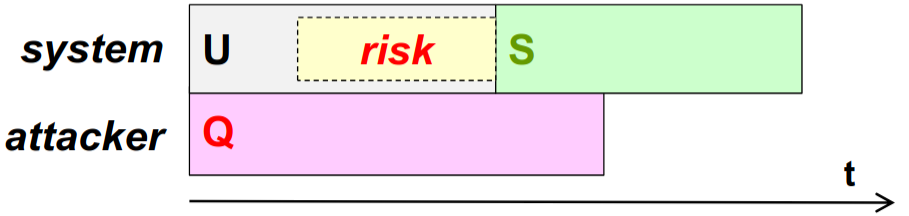
\includegraphics[width=0.6\textwidth]{img/mosca rule.png}
  \caption{Mosca's Rule}
\end{figure}

\section{NIST post-quantum competition}
The emergence of quantum computing has created an urgent need for
cryptographic algorithms that can resist quantum attacks. This is the
essence of \textbf{Moskos' rule}, which emphasizes the importance of
updating cryptographic systems as quickly as possible. To address this
challenge, the \textbf{NIST} launched an international competition in
\textbf{2016} to identify and standardize \textbf{post-quantum
cryptographic} algorithms. These algorithms are also referred to
as \textbf{quantum-resistant} or \textbf{quantum-safe} cryptography.

The selection process began with an open call for nominations, and
several rounds of testing and evaluation were conducted. The
\textbf{first round} concluded with an initial set of proposals. By
\textbf{2019}, a detailed report was published, followed by the start
of the \textbf{third round} in \textbf{2020}, where the most promising
candidates were shortlisted.

For \textbf{public key encryption} (also referred to as a \textbf{key
encapsulation mechanism} or \textbf{KEM}), several algorithms were
shortlisted. Similarly, for \textbf{digital signatures}, three main
algorithms were selected. Unlike traditional cryptographic systems
based on elliptic curves, the shortlisted algorithms are primarily
based on \textbf{structured lattice schemes}, which introduce a new
form of mathematical complexity.

NIST's final selection of PQC algorithms for standardization included
the following:
\begin{itemize}
  \item \textbf{Public Key Encryption (KEM):} 
    \begin{itemize}
      \item \textbf{CRYSTALS-Kyber:} Offers small encryption keys and
        high speed. It is faster than DH and ECDH, making it an
        attractive choice for migration.
    \end{itemize}
  \item \textbf{Digital Signatures:} 
    \begin{itemize}
      \item \textbf{CRYSTALS-Dilithium:} A variant of CRYSTALS with
        robust signature properties.
      \item \textbf{Falcon:} Provides smaller key sizes, offering
        storage and transmission advantages.
      \item \textbf{SPHINCS+:} The only algorithm not based on
        structured lattices. It uses hash functions instead, offering
        a distinct security model. While SPHINCS+ has larger
        signatures and slower computation, it serves as an essential
        fallback option in case structured lattice-based algorithms
        are compromised.
    \end{itemize}
\end{itemize}

In addition to these algorithms, NIST has highlighted several other
candidates for \textbf{potential future standardization}. Most of
these candidates are for \textbf{KEMs} since confidentiality heavily
relies on the secure exchange of keys. Given the critical role of key
exchange in cryptography, ensuring the availability of diverse KEMs is
paramount.

A significant lesson learned from cryptographic history is that
relying on a single mathematical approach can be risky. For example,
attacks on \textbf{integer factorization} led to the transition to
\textbf{elliptic curves}. Similarly, if a vulnerability is discovered
in \textbf{structured lattices}, it could compromise all lattice-based
algorithms simultaneously. This is why \textbf{SPHINCS+}, with its
hash-based construction, is so valuable as it offers a backup method
based on a different cryptographic foundation.

As of the \textbf{fourth round} of the NIST PQC competition, several
new algorithms are being evaluated. Notably, some previously proposed
algorithms have been labeled as \textbf{insecure} due to discovered
vulnerabilities. 

Unlike previous cryptographic advancements (e.g., \textbf{AES} and
\textbf{SHA-3}), where algorithms were tested for years before
standardization, the urgency to protect against quantum threats has
accelerated the process. Standards are being developed and implemented
simultaneously without the luxury of a decade-long evaluation period.
This approach reflects the understanding that quantum computers may
become a reality sooner than anticipated, making it crucial to prepare
and adopt post-quantum cryptographic systems in advance.

\subsection{SIKE}
\textbf{SIKE} (Supersingular Isogeny Key Encapsulation) is a
post-quantum key encapsulation mechanism (\textbf{KEM}) proposed by
\textbf{Microsoft} as part of the \textbf{NIST PQC competition}. It is
part of a family of cryptographic algorithms based on the
\textbf{Supersingular Isogeny Diffie-Hellman (SIDH)} key exchange
protocol. Unlike traditional methods relying on integer factorization
or discrete logarithms, SIKE leverages a novel mathematical approach
involving \textbf{isogenies} between \textbf{elliptic curves}.

SIKE relies on arithmetic operations on \textbf{elliptic curves}
over finite fields. The key idea is to compute \textbf{isogenies},
which are specific types of maps or morphisms between elliptic curves.
The security of SIKE is based on the hardness of finding a particular
isogeny between two elliptic curves. This problem is computationally
challenging and distinct from the traditional \textbf{discrete
logarithm problem} on elliptic curves. In simple terms, while discrete
logarithm problems aim to solve equations like \( g^x \mod p \),
SIKE’s complexity is akin to finding a path within an \textbf{isogeny
graph} of elliptic curves, making it a separate and difficult problem
to attack.

SIKE was implemented by \textbf{Microsoft} and \textbf{Cloudflare} as
a \textbf{constant-time library}. The constant-time approach is
crucial in cryptography to protect against \textbf{time-based
side-channel attacks}. Normally, side-channel attacks attempt to
exploit the time taken by cryptographic operations to leak information
about secret keys. By ensuring that all operations take a constant
amount of time, regardless of the input, SIKE mitigates this risk.

\subsubsection{Hertzbleed Attack}

\textbf{Hertzbleed} is a class of \textbf{frequency-based
side-channel attacks} that exploits \textbf{dynamic CPU frequency
scaling}, a feature found in modern processors like \textbf{Intel
Turbo Boost} and similar technologies on \textbf{AMD Ryzen Zen2 and
Zen3} CPUs. Unlike traditional timing attacks that rely on execution
time differences, Hertzbleed observes the changes in CPU \textbf{clock
frequency} during execution. 

When a CPU encounters computationally intensive tasks, it may adjust
its clock frequency to optimize power and performance. Hertzbleed
exploits this dynamic adjustment to infer information about
cryptographic operations. By analyzing frequency changes, an attacker
can extract information about the execution of cryptographic
algorithms, even when the implementation follows a
\textbf{constant-time execution} principle.

In the worst-case scenario, Hertzbleed could allow an attacker to
\textbf{extract cryptographic keys from remote servers}. This is
because the frequency changes reveal details about the computational
effort required for certain cryptographic operations, allowing
attackers to infer bits of the key. 

Since it is not feasible to "patch" frequency scaling at the hardware
level, \textbf{mitigation requires changes at the software level}.
Possible strategies include:
\begin{itemize}
    \item \textbf{New guidelines for software developers}: Developers
      are advised to avoid operations that could be influenced by
      variable execution times. This includes avoiding arithmetic
      operations whose duration depends on input data.
    \item \textbf{Additional checks and hardening}: Adding additional
      checks to prevent key leakage, but these come with a performance
      penalty. Some cryptographic libraries have been updated to
      follow these guidelines.
\end{itemize}

In the end, besides Hertzbleed, there are other attacks against the
intrinsic math of SIDH so the authors decided to withdraw the proposal
from the NIST PQ competition.

\subsection{NTRU}
Among the algorithms that have not yet been standardized, but they are
very promising, there is the \textbf{NTRU} algorithm. 
It includes two main schemes: NTRUEncrypt, which was patented but
released into the public domain in 2017, and NTRUSign, which remains
patented but can be used in software under the GPL license. One of
NTRU's key strengths is its immunity to Shor's algorithm, making it
resistant to quantum attacks. It also features fast private-key
operations, with complexity scaling quadratically with key size,
unlike RSA, which scales cubically. 

In 2010, NTRU demonstrated impressive performance, being only 20 times
slower than AES-256 at equivalent security strength. As part of the
PQCRYPTO project (H-2020-645622), the provably secure Stehle–Steinfeld
version of NTRU was evaluated. However, this version is less efficient
than the original NTRU. To address structural vulnerabilities, NTRU
Prime was developed to avoid attacks that exploit the algebraic
structures present in the original design.

\subsection{First NIST Standards}

On August 13th, 2024, the first three post-quantum cryptography
standards were introduced. The first standard, ML-KEM (FIPS 203),
stands for Module-Lattice-Based Key-Encapsulation Mechanism, and was
based on CRYSTALS-Kyber. The second, ML-DSA (FIPS 204), is the
Module-Lattice-Based Digital Signature Algorithm, which was based on
CRYSTALS-Dilithium. The third, SLH-DSA (FIPS 206), represents the
Stateless Hash-Based Digital Signature Algorithm, which was based on
SPHINCS+.

\subsection{The FALCON Problem}
The fourth algorithm considered for post-quantum cryptography was
Falcon. Falcon, which is already being prepared for standardization
under draft standard DN-DSA (FIPS 206), stands for Fast Fourier
Transform over N-True Lattice-Based Digital Signature. While Falcon is
a promising signature algorithm due to its speed and use of small
keys, it faces a significant challenge. It requires floating-point
operations as part of the Fast Fourier Transform, and floating-point
operations are difficult to perform in constant time. As a result,
Falcon is heavily susceptible to time-based side-channel attacks.
Currently, NIST and cryptographers are working to find an
implementation that does not exhibit this vulnerability. While the
algorithm is expected to be standardized soon, it is not recommended
for use until this issue is resolved.

\subsection{NIST PQC security levels}
One thing that is changing with PQ is the evaluation of the security:
with traditional cryptography, the security is evaluated in terms of 
the number of bits of the key, but with PQ it's not possible to do
not use keys, but many different parameters that affects the
computation of the ciphertext. To evaluate the security of a PQ 
algorithm, NIST has introduced the concept of \textbf{security
levels}, which are based on the estimated number of operations needed 
to break the algorithm. For example level 1 is something which is
considered equivalent to AES-128 in the sense that if one wants to
attack the algorithm, they need to perform an exhaustive key search
equivalent to the one performed with Grover over AES-128.

\begin{figure}[H]
  \centering
  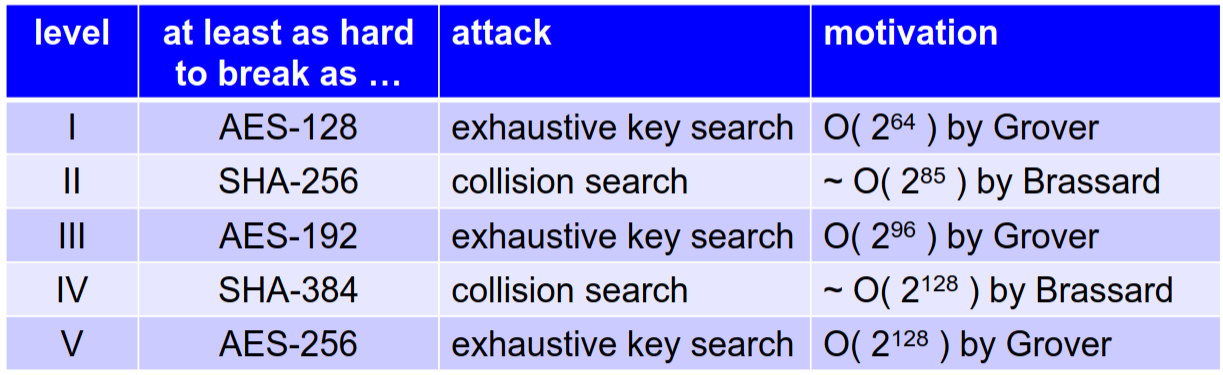
\includegraphics[width=0.6\textwidth]{img/nist security levels.png}
  \caption{NIST PQC Security Levels}
\end{figure}

\subsection{ML-DSA}
ML-DSA is a quantum-resistant digital signature algorithm that
internally uses SHAKE-256 as its cryptographic hash function. The
algorithm's variants are named according to the dimensions of the
\textbf{A} matrix used in its computations. 

The three main versions of ML-DSA are as follows: 
ML-DSA-44, ML-DSA-65, and ML-DSA-87, which correspond to matrix
dimensions of 4x4, 6x5, and 8x7, respectively. 

\begin{figure}[H]
  \centering
  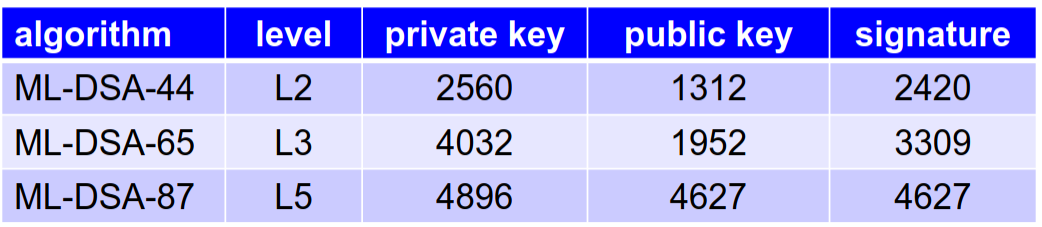
\includegraphics[width=0.6\textwidth]{img/mldsa.png}
  \caption{ML-DSA (sizes in bytes)}
\end{figure}

\subsection{ML-KEM}
ML-KEM is a quantum-resistant key encapsulation mechanism (KEM)
designed to securely encapsulate a symmetric secret key. The
algorithms are identified by specific parameter sets, rather than key
sizes. The main versions of ML-KEM are as follows: 
ML-KEM-512, ML-KEM-768, and ML-KEM-1024. Among these, ML-KEM-768 is
the suggested default for most applications. 

These parameter sets are used to encapsulate a 256-bit (32-byte)
encapsulated key, as per the following table. 

\begin{figure}[H]
  \centering
  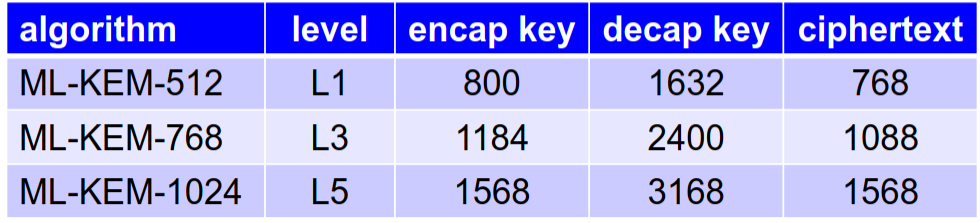
\includegraphics[width=0.6\textwidth]{img/mlkem.png}
  \caption{ML-KEM (sizes in bytes)}
\end{figure}

\subsection{SLH-DSA}

SLH-DSA is a quantum-resistant digital signature algorithm that
combines two signature schemes to ensure robust security. It
integrates both a few-time signature scheme and a multi-time signature
scheme, each playing a distinct role in its operation: 

\begin{itemize}
  \item \textbf{1. Few-Time Signature Scheme:}  The Forest of Random
    Subsets (FORS) is employed to securely sign a limited number of
    messages. This approach ensures that even if multiple messages are
    signed, the security guarantees are not compromised.

  \item \textbf{2. Multi-Time Signature Scheme:}  The eXtended Merkle
    Signature Scheme (XMSS) is utilized as a multi-time signature
    mechanism. XMSS relies on the hash-based one-time signature scheme
    known as Winternitz One-Time Signature (WOTS+), providing robust
    security for multiple signing operations. 
\end{itemize}

Due to its design, SLH-DSA imposes a limit on the number of signatures
that can be generated, which is why a extended Merkle tree is used. It
also makes extensive use of cryptographic hash functions from both the
SHA2 and SHA3 families:  
\begin{itemize}
  \item \textbf{SHA-256} and \textbf{SHAKE-128} are allowed only for
    L1 security.  
  \item \textbf{SHA-512} and \textbf{SHAKE-256} are permitted for all
    security levels.  
\end{itemize}

Another quirk of SLH-DSA is that for each version there are two 
different versions, a \textbf{fast} one and a \textbf{small} (small
signature) one. Furthermore, with the letter $n$ is indicated the 
number of parameters used in the algorithm.

\begin{figure}[H]
  \centering
  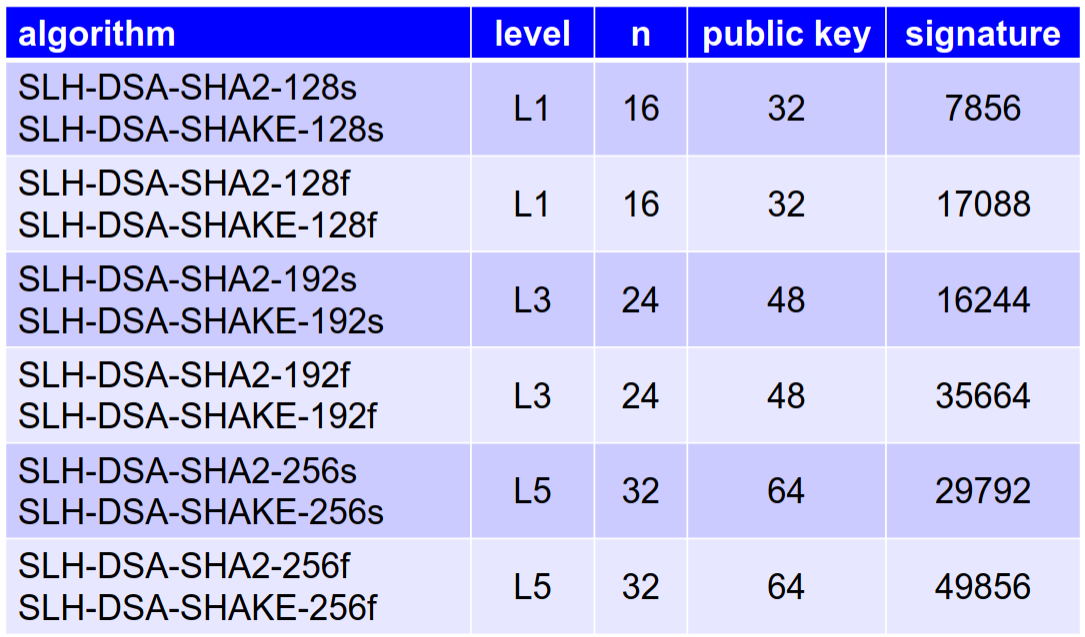
\includegraphics[width=0.6\textwidth]{img/slhdsa.png}
  \caption{SLH-DSA (sizes in bytes)}
\end{figure}

\section{CNSA 2.0 (2022)}

The Commercial National Security Algorithm Suite, version 2 (CNSA 2.0), 
includes the following algorithms: 

\begin{itemize}
  \item \textbf{Symmetric Encryption:} AES-256
  \item \textbf{Flow Mode:} CTR (for low bandwidth) or GCM (for high
    bandwidth)
  \item \textbf{Hash:} SHA-384 or SHA-512
  \item \textbf{Key Agreement:} CRYSTALS-Kyber with level V
    parameters
  \item \textbf{Digital Signature:} CRYSTALS-Dilithium with level V
    parameters
  \item \textbf{Digital Signature of Firmware and Software:} 
    All NIST SP 800-208 algorithms, including LMS and XMSS, 
    with suggested LMS SHA256/192
\end{itemize}

\section{Browsers and Post-Quantum Cryptography}
We have stressed that we have to implement PQ cryptography as soon as 
possible, but in some browsers are "already" implemented. For example,
if you go at \url{https://pq.cloudflareresearch.com/} you can see that 
Cloudflare is already using PQ cryptography for establishing a secure
channel. But if one check which algorithm is used, it's actually
AES-256, and a string like \texttt{X25519MLKEM768} is shown.
\texttt{MLKEM768} is a PQ algorithm, but \texttt{X25519} is not, it's
the insurance against lattices, which are already implemented but have
not yet been thoroughly tested. The approach implemented by Cloudflare 
is to use a hybrid approach, where the key exchange is done with a 
traditional algorithm (\texttt{X25519} is a PQ-DH algorithm) and then
encrypted with a PQ algorithm, meaning that an attacker have to break 
both algorithms to break the encryption.

\section{PQC practical problems}
\begin{itemize}
  \item size of signatures
  \item size of certificates (and certificate chains, which are
    already enormous)
  \item size of network packets
  \item hardware support
  \item "cryptographic agility" against possible attacks
  \item middleboxes (proxy, firewall, IDS/IPS, …)
  \item legacy systems
  \item huge work ahead 
\end{itemize}

\section{Quantum Key Distribution (QKD)}

Quantum Key Distribution (QKD), often mistakenly referred to as
quantum cryptography, is a method for generating a shared secret key
between two parties via a physical channel, typically an optical
fiber, although other mediums are also possible. The key feature of
QKD is that any eavesdropper attempting to intercept the communication
would necessarily disturb the quantum state, thereby revealing their
presence.

QKD relies on quantum mechanics to ensure the secrecy of the key, but
it also requires a classical authenticated side channel for
synchronization and message exchange. However, this requirement
introduces a critical limitation: since the classical channel must be
authenticated, pure QKD in isolation is insufficient for secure
communications. 

There are also technical limitations to QKD systems: 
\begin{itemize}
  \item \textbf{Distance:} Ranges are typically limited to 10 to 100
    km.  
  \item \textbf{Speed:} Key generation rates range from 0.1 to 1 Mbps,
    which is significantly slower than traditional key distribution
    methods. Additionally, since QKD requires 1 bit of key for each
    bit of encrypted data, the bandwidth requirements are
    considerable.  
\end{itemize}

QKD cannot provide end-to-end security but only guarantees
\textbf{hop-by-hop security}. This approach introduces potential
vulnerabilities in intermediary devices, as these "middleboxes" must
be trusted. As a result, QKD is best suited for \textbf{site-to-site
security}, such as securing connections between two data centers.
Despite these limitations, QKD remains a significant area of research
due to its ability to detect eavesdropping, a unique feature enabled
by quantum principles.

\subsection{Quantum Key Distribution (QKD) Protocol}

A QKD protocol requires five key components to facilitate secure key
distribution using quantum principles:

\begin{itemize}
  \item \textbf{Encoding System:} The method used to represent quantum
    information, often using quantum states like photon polarization
    or phase shifts.
  \item \textbf{Source (Alice):} The party responsible for generating
    and sending the qubits (quantum bits) over the quantum channel to
    the receiver (Bob).
  \item \textbf{Quantum Channel and Classical Channel:} The quantum
    channel transmits the qubits (data) between Alice and Bob,
    typically via optical fiber. The classical channel is used for key
    sifting, synchronization, and coordination between Alice and Bob.
    While the quantum channel is susceptible to eavesdropping, the
    classical channel is authenticated to prevent tampering. 
  \item \textbf{Receiver (Bob):} The party receiving the qubits and
    measuring them according to the chosen basis. Measurements
    collapse the quantum state, and any interference by an
    eavesdropper would be detectable.
  \item \textbf{Post-Processing:} After transmission, Alice and Bob
    perform key reconciliation to ensure they have the same key. This
    includes:  
    \begin{itemize}
      \item \textbf{Error Correction:} Corrects any differences in the
        bits caused by noise or other disturbances during
        transmission.  
      \item \textbf{Privacy Amplification:} A method to reduce the
        amount of information an eavesdropper may have obtained about
        the key. If an attacker gains knowledge of some bits of the
        key, Alice and Bob can apply a hash function to reduce the
        key's length, resulting in a shorter but more secure key that
        the attacker cannot reconstruct.  
    \end{itemize}
\end{itemize}

In QKD, a "basis" is the reference system used to handle and measure
qubits. For example, in the BB84 protocol, Alice may randomly select
between two bases (rectilinear or diagonal) to encode the qubits,
while Bob randomly chooses a basis to measure them. If Alice and Bob
use the same basis, they obtain the same bit. If the basis differs,
the result is discarded.

This structure allows QKD to detect the presence of an eavesdropper
and provides a mechanism for securely distributing encryption keys.

\subsection{The BB84 QKD Protocol}

The BB84 protocol is one of the most well-known and widely used QKD
protocols. It leverages the principles of quantum superposition and
the measurement of quantum states to establish a secure shared key
between two parties (Alice and Bob) while detecting potential
eavesdropping.

It operates as follows:
\begin{itemize}
  \item \textbf{Step 1:} Alice selects random polarization states to
    send her bits. Each bit is encoded into a quantum state (qubit)
    using one of two possible bases (e.g., rectilinear or diagonal).

  \item \textbf{Step 2:} Bob uses random polarization states to detect
    the qubits sent by Alice. Since Bob does not know Alice's basis in
    advance, he randomly chooses a basis for each bit measurement.

  \item \textbf{Step 3:} Bob informs Alice of the polarization states
    he used to measure the qubits (but not the measurement results). 

  \item \textbf{Step 4:} Alice tells Bob which bits were measured
    using the correct polarization basis. These bits are retained,
    while the others are discarded. This process is known as
    \textbf{sifting}.
\end{itemize}

Even after sifting, there may be errors in the shared bits. Errors can
occur due to an imperfect quantum channel or interference caused by an
eavesdropper (Eve). To address these errors, Alice and Bob apply error
correction codes to reconcile their bits and ensure they have
identical shared keys.

After the error correction phase, the proportion of bits that remain
valid compared to the total transmitted bits defines the
\textbf{Quantum-Bit Error Rate (QBER)}. The number of valid bits is
significantly less than the total number of bits originally
transmitted.

\begin{figure}[H]
  \centering
  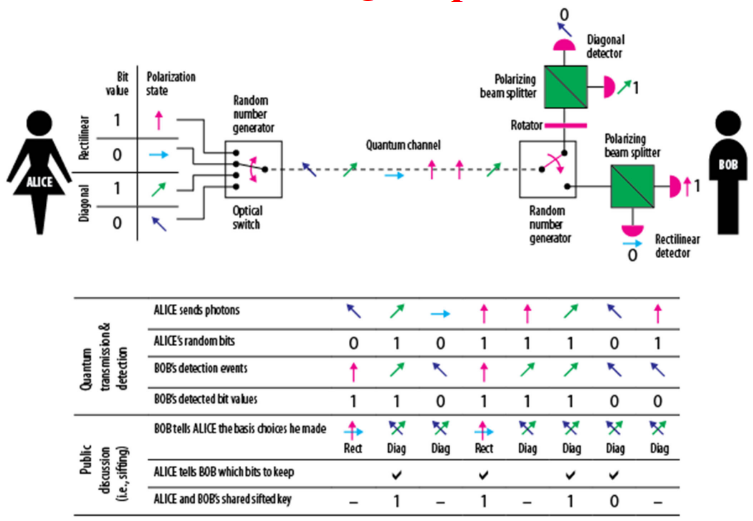
\includegraphics[width=0.6\textwidth]{img/bb84.png}
  \caption{BB84 Protocol}
\end{figure}

\subsection{The Photon Number Splitting (PNS) Attack}

The Photon Number Splitting (PNS) attack is an active attack that
exploits imperfections in the devices used for the practical
implementation of QKD protocols like BB84. This attack specifically
targets the source, known as Alice, which is responsible for
generating qubits.

Eve, the attacker, takes advantage of the fact that Alice's source
does not always produce single-photon pulses. By counting the number
of photons in each pulse, Eve can choose how to act. If the pulse
contains only one photon (\(N = 1\)), she blocks it entirely. However,
if the pulse contains multiple photons (\(N > 1\)), Eve stores one
photon and forwards the remaining photons to Bob. This allows her to
extract part of the quantum information while remaining undetected.

The attack further exploits the basis information exchanged between
Alice and Bob during the sifting phase of the BB84 protocol. Since
this exchange happens over a classical authenticated channel that
guarantees authenticity but not confidentiality, Eve can use the
disclosed basis information to measure the stored photons correctly.
This flaw in the protocol allows Eve to extract additional information
about the key.

The core vulnerability of this attack lies in the inability of
practical QKD sources to guarantee single-photon pulses. Multi-photon
pulses provide Eve with an opportunity to intercept and measure part
of the quantum information. This attack poses a significant threat to
the security of QKD systems, especially when the photon source is not
perfectly isolated to emit only single photons.

\subsection{The Decoy State Protocol}

The Decoy State protocol is a modification of the BB84 QKD protocol
designed to counter the Photon Number Splitting attack. It introduces
a mechanism to detect the presence of an eavesdropper by varying the
intensity of the pulses sent from Alice to Bob.

In this protocol, Alice sends pulses of different types, all having
the same wavelength, duration, and shape but with varying intensities.
Some of these pulses carry actual quantum information, while others
are decoy pulses. The key idea is that, from the perspective of an
eavesdropper like Eve, there is no obvious way to distinguish the
decoy pulses from the information-carrying pulses.

After transmission, Alice and Bob disclose the basis and the type of
each pulse. By comparing the number of decoy pulses sent to the number
of decoy pulses received, they can detect anomalies that may indicate
the presence of a PNS attack. If Eve attempts to intercept and measure
these pulses, the discrepancy between the sent and received decoy
pulses will reveal her presence.

The Decoy State protocol significantly enhances the security of QKD
systems by making it much harder for an attacker to exploit
multi-photon pulses. By using decoys, the system introduces
uncertainty for the attacker, thereby mitigating the risks posed by
the imperfections of practical quantum sources.

\subsection{Other types of QKD protocols}
Other types of QKD protocols are possible and being developed, which
mostly leverage entanglement. Rather than having Alice to prepare and
send and Bob to measure the results, the two parties share an 
Entangled Source in the quantum channel, and since the qbits are 
entangled, one can infer the state of the other. This means that the
two parts are able to share a random key, which is generated
automatically.

Once the key has been generated, it can be used either as key for
classical symmetric encryption, or as key for a one-time pad. 

\section{One-Time Pad} 

One-time pad encryption is a theoretically perfect secret key
encryption algorithm, offering absolute security when implemented
correctly. The core requirement for this method is the use of a
"one-time pad," which is a pre-shared, single-use key that is as large
as or larger than the message it encrypts.

The encryption process works by combining each unit of plaintext (bit,
byte, or character) with the corresponding unit of the one-time pad.
This combination is typically done using modular addition, most
commonly implemented as an XOR operation. The result is a ciphertext
that is computationally indistinguishable from random noise, ensuring
perfect secrecy.

A significant advantage of one-time pad encryption is its ability to
achieve unbreakable encryption under ideal conditions. However,
practical challenges arise from the need for a pad that is at least as
long as the message and from the requirement that each pad must only
be used once. Reusing a pad can lead to vulnerabilities and compromise
security.

QKD can address some of these practical issues, enabling the secure
on-the-fly distribution of the shared key, eliminating the need to
pre-share it. Additionally, QKD can create a "key pool" from which
bits can be extracted as needed. However, using a key pool poses
certain risks, as improper key management or reuse can undermine the
perfect secrecy guaranteed by the one-time pad.

The general schema is shown in the figure \ref{fig:otp}. As you can
see, it's a simple xor between the plaintext and the key.

\begin{figure}[H]
  \centering
  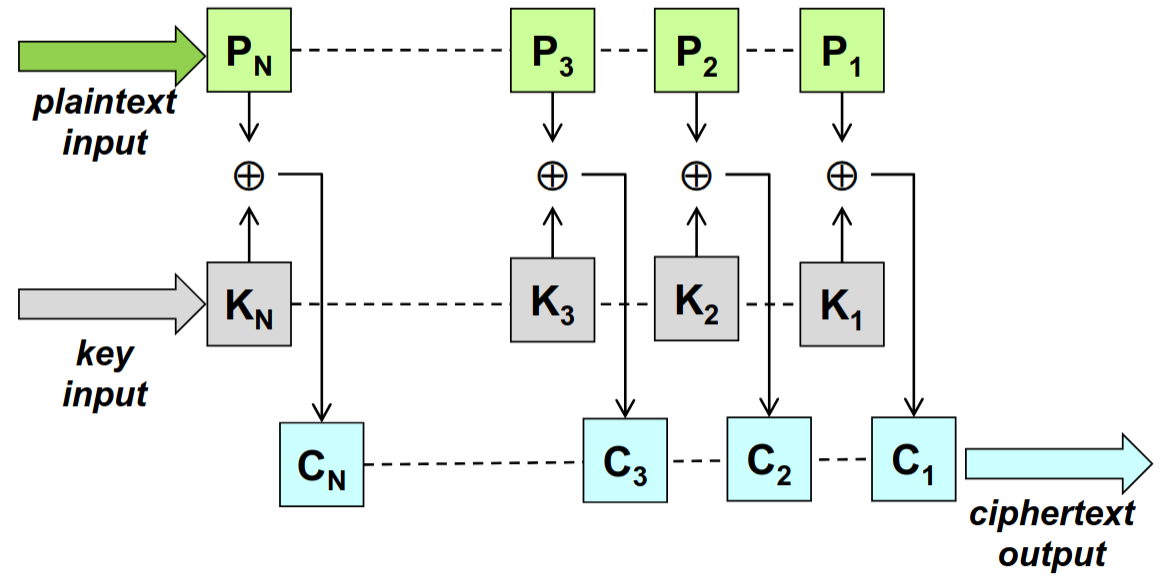
\includegraphics[width=0.6\textwidth]{img/otp.png}
  \caption{One-Time Pad encryption}
  \label{fig:otp}
\end{figure}

\subsection{Key Requirements}

The security of a OTP encryption scheme relies heavily on the
properties and management of its key. To ensure perfect secrecy, the
key must meet the following stringent requirements.

First, the key must be at least as long as the plaintext. This is a
fundamental condition to guarantee that each unit of the plaintext
(bit, byte, or character) has a unique corresponding key unit with
which it can be combined, typically using an XOR operation.

The key must also be genuinely random. This means it must be uniformly
distributed across the set of all possible keys and entirely
independent of the plaintext. True randomness requires the use of a
non-algorithmic, chaotic source, such as a hardware-based random
number generator (RNG). Merely passing statistical randomness tests is
not sufficient, as these tests can be deceived by pseudo-random
sequences. According to Gregory Chaitin's definition, the key should
be patternless, meaning it must not exhibit any discernible structure
or predictability.

Another essential requirement is that the key must have a number of
bits of entropy at least equal to the number of bits in the plaintext.
If the entropy is lower, an attacker could attempt to reconstruct the
key by attacking the RNG algorithm that generated it.

The key must never be reused, in whole or in part. Reusing any portion
of the key introduces vulnerabilities, as attackers could analyze
ciphertexts encrypted with the same key material to extract
information about the plaintext.

Finally, the key must be kept entirely secret from any unauthorized
parties. If an attacker gains access to the key, the security of the
encryption is completely compromised. Unlike other cryptographic
methods, there is no fallback protection in the one-time pad system if
the key is exposed.

\subsection{Practical problems}
\begin{itemize}
  \item size of the one-time pad (distribution and storage problems)
  \item true randomness of the one-time pad values (values generated by
    PRNG can be predicted)
  \item secure generation of the one-time pad values (real-time RAM /
    CPU attacks, or forensic analysis)
  \item secure exchange of the one-time pad values (MITM / MATE attacks)
  \item secure use of the one-time pad values (real-time RAM / CPU
    attacks)
  \item secure disposal of the one-time pad values (forensic analysis)
\end{itemize}

\subsection{Key Combiner}

A key combiner is a mechanism used to merge multiple shared secrets
into a single, stronger secret. The main advantage of this approach is
that even if one of the shared secrets is compromised, the resulting
combined key remains secure. The combination of secrets can be
represented as:
\[
ss = \texttt{keyCombiner}(ss_1, ss_2, \ldots, ss_N)
\]
where \(ss_1, ss_2, \ldots, ss_N\) are the individual shared secrets.

These shared secrets can be obtained through various methods, such as:
\begin{itemize}
    \item \textbf{Agreed secrets}: Derived through key exchange
      protocols like Diffie-Hellman (DH).
    \item \textbf{Distributed secrets}: Distributed using asymmetric
      encryption methods, such as RSA or Key Encapsulation Mechanisms
      (KEM).
    \item \textbf{Pre-shared secrets}: Keys that are established
      before the communication begins.
    \item \textbf{On-the-fly generated secrets}: Keys generated
      dynamically using techniques like Quantum Key Distribution
      (QKD).
\end{itemize}

One of the most promising key combiners is the \textbf{X-wing
combiner}, which is specifically designed to mix keys obtained from
QKD with other types of keys, enhancing the overall security of the
combined key.

\subsection{ETSI QKD network}
The ETSI group have been proposing many standard to use QKD for
networking. Take a look at the figure \ref{fig:etsi} to see a possible
network configuration. It presents some Sites (A, B and C) with two
QKD links between them, managed by quantum key distribution devices,
or endpoints. The keys generated or distributed by these devices are
managed by a key management entity, which are critical components and
as such are very protected. ETSI has also standardized a key delivery
API, in which an application, which they call it Secure Application
Entity or SAE, can request to have a key stream, which is synchronized
with another application running on a corresponding site. This
means that this key management entity will synchronize its work with
this other key management entity, and they will provide the same bits
to the two applications that then can perform encryption, for example,
with a one-time pad

